\documentclass[11pt,a4paper]{article}

\usepackage[T1]{fontenc}

\usepackage[margin=25mm]{geometry}

\usepackage{booktabs,tabularx,longtable,amsmath,hyperref}

\usepackage{pgfplots}

\pgfplotsset{compat=1.18}

\usepgfplotslibrary{groupplots}

\hypersetup{colorlinks=true,urlcolor=blue,linkcolor=black}

\setlength{\parskip}{5pt}

\setlength{\parindent}{0pt}

\emergencystretch=3em

\title{An Empirical Evaluation of Shepherd TypeScript\\[5pt]\large Durable execution, reliability, a matched harness comparison, and context selection}

\author{Repository benchmark study}

\date{5 October 2026}

\begin{document}\maketitle

\begin{center}\small Technical report: single-host systems study and local-model pilot\end{center}

\begin{abstract}

Reversible agent runtimes require evaluation of durable operations, state preservation, and model behavior as distinct properties. We evaluate Shepherd TypeScript runtime 12.0.3 on an Apple M4 Pro with APFS, using three fresh-dataset kernel repetitions, one complete scope experiment, checkpoint and device-layer measurements, and a 96-call local-model experiment. The median of kernel run medians is 0.237 ms for durable single-record append and 4,338.863 records/s for sequential append throughput. All 30 kernel budget comparisons pass. The scope experiment passes 150 recorded restoration checks but misses one of 17 latency budgets. A separate carrier-storage assertion fails; zero and coarse free-space deltas invalidate precise storage-efficiency claims from this run. A matched direct invocation harness and Shepherd send identical requests to Qwen2.5-Coder 0.5B and return identical outputs in all 48 pairs. Relevant-evidence selection raises joint answer-and-citation success from 0/16 to 14/16 per harness while reducing mean prompt length from 1,403 to 233 tokens. All 48 Shepherd terminal sessions preserve their result through command repetition, store reopen, and archive import. These results establish bounded local evidence for durable execution and context sensitivity, not a ranking of independent frameworks, general coding competence, or reproduction of upstream application results.


\end{abstract}

Keywords: Agent runtimes; reversible execution; durable traces; benchmarking; reliability; context engineering; evidence-grounded generation


\section{Introduction}

An agent runtime can be fast without preserving recoverable state, and an agent can finish a conversation without solving its task. A benchmark that reports only wall-clock duration or terminal status conflates these outcomes. This study therefore treats execution cost, retained-state correctness, and independently judged task output as separate dependent variables. Its subject is the Shepherd TypeScript repository, an independent implementation of reversible, inspectable execution over a language-neutral protocol [1, 2].


The runtime organizes execution around tasks, effects, scopes, and traces. For the local implementation, the experimentally relevant interfaces include SQLiteTraceStore, forkScope and discardScope, replay sessions, checkpoint adapters, provider invocations, and trace subscriptions. A physical filesystem branch, a public durable scope fork, and a replay checkpoint have different contracts. Measuring one operation does not establish the latency or recovery semantics of the others.


The requested evaluation spans four areas: performance and reliability; comparison with another harness; model-backed task quality; and context engineering. We address the first with existing repository procedures and fresh observations. We address the second with a deliberately minimal direct harness using the same provider adapter and requests. We address the remaining areas with a controlled, synthetic evidence-grounding pilot using an installed local model. Independent third-party frameworks are discussed as related work, not presented as experimentally ranked competitors.


The contribution is an auditable local study rather than a new runtime design: retained samples and configurations, explicit timing boundaries, a matched request control, an executable answer-and-evidence judge, result retention checks at public persistence boundaries, and a report that preserves negative findings. Production code, benchmark procedures, dependencies, and SLO budgets are unchanged. The report is packaged as documentation release 13.7.1; the measured runtime identifies itself as 12.0.3. Publication is based on main 13.7.0; the newer runtime is not the subject of these measurements.


\section{Background and Related Work}

The Shepherd paper motivates programmable operations over agent executions and studies substrate costs, cache reuse, and meta-agent applications [1]. Its sandbox readiness boundary differs from the local TypeScript public API boundary, which includes durable custody publication and verification. We therefore borrow research dimensions, not numerical baselines. The pinned Python implementation and its separately maintained experiment repository are useful methodological references, but their existing kernel and sandbox workloads do not perform the same work as this study [3].


AgentGit studies Git-like workflow history and branching for LangGraph-based workflows [4]. The OpenHands Software Agent SDK emphasizes extensible agents, tools, memory, and execution lifecycle [5]. BranchFS concerns filesystem branch contexts [6], while StateFork distinguishes logical exploration from physical materialization [7]. These works identify relevant design axes; their presence in the bibliography does not establish feature parity or superiority. No executable from these projects was run in the present comparison.


A valid independent-framework experiment must harmonize task inputs, tools, provider settings, durability, restored constituents, resource budgets, and timing start and stop conditions. Upstream experiment inspection found cloud and Linux/overlay dependencies and different operation semantics. Rather than divide incomparable published latencies, the present control isolates the local cost and behavior of adding a durable replay-session boundary to an otherwise identical provider invocation. The direct control is implemented by this study and shares Shepherd's provider adapter, so it is not an independent implementation of that adapter.


SQLite durability is part of the workload. In WAL mode, synchronous FULL introduces a WAL synchronization at transaction commit [8]. A volatile or differently synchronized baseline would deliver a different guarantee. Similarly, copy-on-write storage behavior depends on the filesystem and write pattern. A label such as clone or overlay does not make an API constant-time when that API also verifies content.


\section{Research Questions}

RQ1: What are the local costs of durable append, causal-prefix resolution, subscriptions, archive interchange, integrity verification, and CLI startup under the fixed kernel workload? RQ2: How do scope fork and revert costs change with world size and available carrier backend, and do the observed restoration checks pass? RQ3: Are storage and checkpoint measurements sufficiently valid to support representation-efficiency claims?


RQ4: Does the durable session harness change outputs when paired with a direct harness on identical provider requests, and what client-side work remains outside the HTTP transport interval? RQ5: How do complete, selected, and incomplete evidence packages affect answer accuracy, citation accuracy, abstention, prompt length, and completion? RQ6: Does retained terminal evidence survive command repetition, store reopen, and archive import, including failed model invocations?


These questions concern observable operations and task criteria. They do not ask whether the model learns from reversibility, whether context retrieval is generally optimal, whether arbitrary process images restore, or whether a framework is safe under all failures. Those claims require additional experiments and distinct evidence.


\section{Experimental Method}

\subsection{Host, source, and execution conditions}

All fresh system measurements use one Apple M4 Pro host: 14 CPU cores, 48 GiB memory, Darwin 27.0.0, APFS filesystem type 26, Node.js 24.17.0, and bundled SQLite 3.53.0. The source revision is d7f957caacd1e57e40417d42587618f702b5e8ca. The checkout contains earlier uncommitted documentation and release-metadata work, recorded in provenance.json. The initial diff over src, scripts, tooling, config, and protocol.config.json is empty; this is not described as a clean checkout.


System suites execute serially. The three kernel repetitions create fresh scratch stores and datasets within one long-lived Node process; they are not independent process, host, or machine replicates. JIT and OS cache state can carry across repetitions. The model experiment follows the system suites. A six-call smoke experiment is retained separately and excluded from all reported task counts. It can warm the model and prompt cache. The host is not dedicated or load-isolated, and background activity is neither measured nor controlled.


The study uses a local Qwen2.5-Coder 0.5B model, metadata size 494.03M parameters, GGUF Q4\_K\_M, served by Ollama 0.35.1. Its recorded model digest is 4ff64a7f502a08b7616edb8ca0a79eb1853fc363d842b7df4b46915d11a3fb09. The metadata advertises a 32,768-token context capacity; the active server window is not pinned or independently verified. The largest mean measured prompt is 1,403 tokens. The local OpenAI-compatible endpoint receives temperature 0.2, seeds 17 and 43, a 128-token completion cap, and a 120-second client deadline. The transport maps the output cap to max\_tokens; its exact bodies are retained. No remote model or paid API is used [9].


\subsection{Kernel and scope workloads}

The unmodified kernel configuration creates 40 regular owners with 200 records each and a 2,000-record deep owner, for 10,000 semantic dataset records. Records contain 256 padding characters and cite their predecessor. Each owner has two cuts. The fixture also contains 40 registered 1 KiB blobs, 20 orphan blobs, and four abandoned temporary files. Each of ten metrics performs two unrecorded warmups and 12 recorded samples. Append throughput times 100 sequential single-record appends. Archive export and integrity measurements occur after the append measurement workload, while the import archive was captured before it; these are not exactly identical record counts.


One complete scope experiment measures every carrier reported conformant locally: copy and clone. The worlds contain 10 x 3,072-byte files, 100 x 102,400-byte files, and 100 x 1,048,576-byte files: 30 KiB, approximately 9.77 MiB, and 100 MiB. Fork and revert use two warmups followed by ten recorded samples per backend and world. Fork timing covers forkScope through custody publication and verification. Revert timing covers discardScope after a child write. The experiment also measures K=4 branching with five parent writes and three sibling writes, three repetitions per storage cell, and a four-point mutation-size sweep.


Restoration evidence compares independent SHA-256 tree digests of the source, parent, and a fresh checkpoint fork, checks the fresh custody content identity, and checks that discarded custody no longer opens. The 150 recorded checks are assertion outcomes, not 150 independent failure trials or a probability estimate. The digest helper covers regular-file paths and bytes; it is not a comprehensive metadata, process, or future-observation equivalence test. Observation cells use three sessions at each of 1, 10, 50, 100, and 200 events with 0, 1, or 4 pull observers. Every observer drains after each event. These event timings are nested within sessions.


\subsection{Storage, checkpoints, and application fixtures}

The carrier suite tests 16 and 64 MiB worlds, one or four 1 MiB file replacements, and five repetitions per cell. It measures the filesystem-wide free-space delta after sync and retains a per-cell median, not all underlying storage samples. The scope storage suite similarly uses volume free-space deltas, reports trace-store growth separately, and clamps negative observed deltas to zero. These measurements can include unrelated volume activity and allocator/reporting effects; they require plausibility checks before interpretation.


Automatic-checkpoint storage compares the same deterministic 32-step workflow without checkpoints and with an every-step policy. Four cells combine 16 or 256 files of 4 KiB with one or eight files changed per step. The difference in closed database and content-addressed blob footprint, divided by 32 checkpoints, is the measured overhead. Each cell is one paired workflow experiment, not 32 independent workload replications.


Device-layer timing measures checkpoint and restore after writes over 1, 16, and 128 MiB worlds with two warmups and seven measured steps. Its nearest-index empirical p90 is the largest observation at this sample size. The existing script emits summaries rather than every latency sample, so we do not derive confidence intervals from it. Overlay and container depth experiments are not available in this lane. Separately, the repository's four scripted application fixtures are rerun as conformance evidence. Their configured provider usage and monetary figures are synthetic accounting values, not measured commercial costs or real-model quality.


\subsection{Matched harness and context treatments}

Eight synthetic tasks ask for the current value of one project property, such as a region, retry limit, runtime version, or owner. Each has an obsolete revision-1 document and a current revision-2 document. The instruction requires the value from the highest revision and exactly the supporting document ID. The response schema requires answer and evidence. Ground truth is defined in agent-study.config.json and is never supplied as a separate answer field to the model.


Full context supplies both relevant documents between two blocks of 12 unrelated records, for 26 documents. Selected context supplies only the two relevant documents. Incomplete context supplies the 24 unrelated records and omits both relevant ones; its criterion is answer=null and evidence=[]. This last cell is an abstention stress test, not the same knowledge-access condition as full or selected context. Selection is an oracle lookup over the known synthetic task specification. It is not learned retrieval, summarization, a production context manager, or an evaluation of retrieval recall. Selection overhead is not included in timed provider execution.


Every task runs at both seeds in all three conditions through both harnesses: 8 x 2 x 3 x 2 = 96 calls. The direct harness calls createLiveProvider.invoke. The Shepherd harness runs one context.invokeProvider step through runReplaySession in a file-backed SQLiteTraceStore. Both use the same adapter, prompt, schema, model, transport, and decoding controls. Order alternates within paired cells. The SHA-256 digest of the final HTTP body is checked for equality in every pair. Timing starts after provider/options setup and, for Shepherd, after store creation. It ends after the normalized response or terminal inspection; it excludes judge execution, repetition checks, reopen, and import.


This is a bounded single-invocation agent-workload proxy. It does not run a tool-use policy, autonomous file editing, multi-agent cooperation, or an external coding benchmark. The comparator is another minimal harness authored for this study, not LangGraph, OpenHands, or upstream Python Shepherd. Shared provider code improves request matching but prevents an independent test of that adapter's correctness.


\subsection{Metrics, statistical treatment, and reliability boundaries}

We separately count finished invocations, schema-valid outputs, correct answers, correct evidence sets, and joint success. A strict success requires a finished invocation, the exact configured value, and exactly the current document ID; extra or obsolete citations fail evidence correctness. For incomplete context, correct abstention requires null and an empty evidence list. An independent Python analysis recomputes joint scores from retained outputs. HTTP responses and usage are retained even when a completion hits its token cap and the provider adapter rejects its stop reason.


Prompt length is the server-reported prompt\_tokens, including cached tokens. Shepherd's normalized inputTokens excludes cacheReadInputTokens, so prompt size must not be inferred from inputTokens alone. Cached and uncached accounting are reported separately. Local cache state is retained and shared; most second requests in a pair reuse almost the entire prefix. Missing cache-creation accounting is not interpreted as evidence that no cache was created. Monetary cost remains unavailable. Client residual latency is total measured API time minus HTTP transport time; it includes parsing, validation, and, for Shepherd, trace/session work. It is a diagnostic residual rather than a standalone CPU or durability timer.


Kernel tables report the median of three run medians, their observed range, and the largest per-run empirical p95. Nearest-rank p95 from 12 or 10 samples equals that run's maximum. We do not pool all samples as independent machines or infer a production tail distribution. For the context effect, a task-cluster bootstrap resamples eight whole tasks, retaining both seeds and paired treatments, for 10,000 draws with seed 20261005. Its percentile interval describes sensitivity to this small synthetic battery; it is not a confidence guarantee for unseen coding tasks.


Every Shepherd terminal session is repeated under the same command ID and checked for no additional provider request and the same canonical terminal result. The store is closed and reopened after each session, and the retained terminal result is compared. At the end, its archive is imported into a fresh store, all terminal results are compared, and both stores undergo integrity verification. Failed terminals have null results: equality of null alone is weak evidence for failure-detail preservation. These checks establish result retention and idempotent terminal reuse, not recovery from an in-flight crash or exact-once external side effects. Existing crash/conformance tests provide separate, explicitly scoped evidence.


\section{Results: Runtime Performance and Storage}

\subsection{Durable kernel operations}

Table 1 reports fresh kernel measurements. Durable append has a median-of-medians of 0.237 ms, with run medians spanning 0.201-0.264 ms. Sequential throughput spans 3,898.505-4,431.316 records/s in run medians. Archive export and import are approximately 1.21 s and 1.94 s respectively under this fixture. Resolving the deep owner's cut takes 78.244 ms; materializing a regular 200-record owner prefix takes 7.531 ms. These values apply to their defined workloads, not arbitrary trace sizes.


All ten existing kernel budgets pass in every repetition: 30/30 comparisons. The SLO is a configured regression bound with broad headroom, not an external performance standard or a statistical superiority test. Passing it does not establish scalability beyond the configured trace or reproduce the historical reference figures. We do not attribute differences from previous repository runs to code changes because system load and temporal conditions are uncontrolled.


\begin{center}\small

\textit{Table 1. Kernel results: three fresh-dataset repetitions, 12 samples per metric per repetition.}\[6pt]

\begin{tabularx}{\linewidth}{XXXXX}

\toprule

\textbf{Operation} & \textbf{Unit} & \textbf{Median of medians} & \textbf{Run median range} & \textbf{Largest run p95} \\

\midrule

append latency ms & ms & 0.237 & 0.201-0.264 & 0.340 \\

append throughput records per second & records/s & 4,338.863 & 3,898.505-4,431.316 & 4,656.605 \\

cut resolve ms & ms & 78.244 & 77.196-78.929 & 85.571 \\

slice read ms & ms & 7.531 & 7.448-7.600 & 9.448 \\

subscription pull ms & ms & 7.810 & 7.668-8.180 & 9.662 \\

export ms & ms & 1,210.095 & 1,184.644-1,217.992 & 1,344.787 \\

import ms & ms & 1,941.849 & 1,927.505-1,953.478 & 2,153.220 \\

verify ms & ms & 708.786 & 673.820-709.402 & 760.791 \\

gc inspect ms & ms & 3.317 & 3.096-3.666 & 3.944 \\

cli startup ms & ms & 97.673 & 90.076-100.239 & 117.702 \\

\bottomrule\end{tabularx}\end{center}

\subsection{Scope latency, restoration, and observation}

Table 2 and Figure 1 show that public fork latency increases across the configured worlds for both copy and clone. Copy medians grow from 158.730 ms to 1,100.234 ms; clone medians grow from 174.551 ms to 1,292.423 ms. Clone is not a faster public fork in these cells. Content verification and custody publication are included, so the result does not isolate filesystem clonefile latency or disprove copy-on-write storage behavior. File count changes from the small to medium world, preventing attribution solely to bytes.


All 150 recorded restoration checks pass. However, clone revert on the medium world has empirical p95 314.139 ms against an unchanged 250 ms budget, a 25.7\% exceedance. The other 16 scope budgets pass. The correctness suite's successful exit and the failing SLO comparison are distinct results. We retain the miss rather than expand the budget or select a better rerun. A single noisy cell does not identify a code regression or its cause.


At 200 events, record medians are 0.669 ms with no observers, 0.674 ms with one, and 0.879 ms with four. Subscription-pull medians are 0.147 and 0.150 ms for one and four observers. The four-observer record median is approximately 31.4\% above the zero-observer median in this run, despite observers remaining passive readers. No causal claim is made about the difference. The stream contains two records per event and 2,746.775 JSON bytes per event in every 200-event cell. Record-count equality holds at all configured step counts; it does not alone prove equivalence of complete model contexts.


\begin{center}\small

\textit{Table 2. Public scope latency (ms). Worlds: small 30 KiB/10 files; medium 9.77 MiB/100; large 100 MiB/100. Empirical p95 is the sample maximum.}\[6pt]

\begin{tabularx}{\linewidth}{XXXXXX}

\toprule

\textbf{Backend} & \textbf{World} & \textbf{Fork median} & \textbf{Fork p95} & \textbf{Revert median} & \textbf{Revert p95} \\

\midrule

copy & small & 158.730 & 174.010 & 43.585 & 51.225 \\

copy & medium & 785.271 & 981.714 & 122.687 & 140.240 \\

copy & large & 1,100.234 & 1,287.515 & 206.755 & 264.182 \\

clone & small & 174.551 & 190.753 & 43.637 & 51.119 \\

clone & medium & 1,241.832 & 1,996.053 & 163.893 & 314.139 \\

clone & large & 1,292.423 & 1,331.762 & 201.303 & 206.448 \\

\bottomrule\end{tabularx}\end{center}

\begin{center}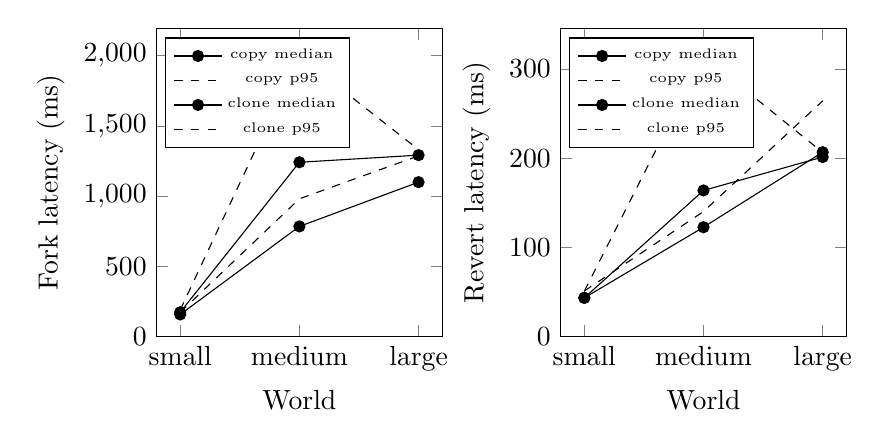
\begin{tikzpicture}

\begin{groupplot}[group style={group size=2 by 1,horizontal sep=1.5cm},width=.43\linewidth,height=5.5cm,legend style={font=\tiny}]

\nextgroupplot[xlabel=World,ylabel={Fork latency (ms)},xtick={0,1,2},xticklabels={small,medium,large},ymin=0,legend pos=north west]

\addplot[mark=*] coordinates {(0,158.73) (1,785.271) (2,1100.234)};

\addlegendentry{copy median}

\addplot[dashed] coordinates {(0,174.01) (1,981.714) (2,1287.515)};

\addlegendentry{copy p95}

\addplot[mark=*] coordinates {(0,174.551) (1,1241.832) (2,1292.423)};

\addlegendentry{clone median}

\addplot[dashed] coordinates {(0,190.753) (1,1996.053) (2,1331.762)};

\addlegendentry{clone p95}

\nextgroupplot[xlabel=World,ylabel={Revert latency (ms)},xtick={0,1,2},xticklabels={small,medium,large},ymin=0,legend pos=north west]

\addplot[mark=*] coordinates {(0,43.585) (1,122.687) (2,206.755)};

\addlegendentry{copy median}

\addplot[dashed] coordinates {(0,51.225) (1,140.24) (2,264.182)};

\addlegendentry{copy p95}

\addplot[mark=*] coordinates {(0,43.637) (1,163.893) (2,201.303)};

\addlegendentry{clone median}

\addplot[dashed] coordinates {(0,51.119) (1,314.139) (2,206.448)};

\addlegendentry{clone p95}

\end{groupplot}\end{tikzpicture}

\par\small\textit{Figure 1. Median and empirical p95 public scope latency. Both file count and bytes change between small and medium; timing includes custody publication and verification.}\end{center}

\subsection{Storage measurement failure and checkpoint representation}

The standalone carrier suite exits with an assertion failure: a copy branch over a 16 MiB world with 1 MiB replaced reports zero growth, below its configured minimum. Scope storage medians also contain zeros and coarse 40,960,000-byte jumps, even when the independently measured trace-store growth is 510,880 bytes. These observations are not credible evidence of free storage. The precise cause, such as reporting lag or unrelated volume activity, is not diagnosed. The clamping of negative deltas further limits interpretation.


The raw mutation sweep remains available, including fitted storage slopes and R-squared values, but those regressions are not promoted to physical-efficiency claims because their input measure failed plausibility checks. In particular, we do not report a precise clone-versus-copy storage saving from these measurements. Direct allocated-block accounting or an isolated test volume with stable baseline readings is needed before such an effect is estimated.


Automatic-checkpoint storage uses a different measure: closed file footprints. Table 3 shows 17,393 bytes per checkpoint for a 16-file world changing one 4 KiB file per step, and 93,825 bytes for a 256-file world with the same changed byte count. The approximately 5.39-fold increase is consistent with the workload's full manifest and metadata cost; it is not a full-world byte copy claim. Increasing changed files to eight raises the corresponding totals to 48,241 and 124,929 bytes. One paired execution per cell supports these observed totals without a sampling interval.


\begin{center}\small

\textit{Table 3. Additional storage per automatic checkpoint, computed from one 32-step paired workflow per cell. Every file is 4 KiB.}\[6pt]

\begin{tabularx}{\linewidth}{XXXXX}

\toprule

\textbf{World files} & \textbf{Changed files/step} & \textbf{Blob bytes} & \textbf{DB bytes} & \textbf{Total bytes} \\

\midrule

16 & 1 & 8,817 & 8,576 & 17,393 \\

16 & 8 & 36,593 & 11,648 & 48,241 \\

256 & 1 & 81,537 & 12,288 & 93,825 \\

256 & 8 & 109,313 & 15,616 & 124,929 \\

\bottomrule\end{tabularx}\end{center}

\subsection{Device-layer costs and unavailable lanes}

Table 4 records device-layer checkpoint and restore summaries for copy and clone. Copy checkpoint medians are 90.16, 1,139.38, and 9,400.98 ms over 1, 16, and 128 MiB. Clone medians are 130.84, 1,593.85, and 13,484.88 ms. The largest/smallest checkpoint ratios are 104.27 and 103.06 over a 128-fold world-size increase. File count scales with bytes in this workload, so the experiment does not distinguish content-volume cost from per-file work.


Overlay is unavailable on this platform and the container probe reports container-daemon-unavailable in the sandboxed execution lane. Neither adapter is measured, and the configured depth sweep consequently has no rows. The absence of depth data or a skipped constant-ratio assertion is not a pass for constant-time checkpointing. Device-layer operations here do not establish scope-fork latency, replay-checkpoint atomicity, arbitrary process restoration, or durable layer recovery after restart. Historical Linux/container figures remain separate evidence and are not relabeled as fresh observations.


\begin{center}\small

\textit{Table 4. Device-layer summaries in ms: seven measured steps per cell. Empirical p90 equals the maximum; underlying latency samples are not emitted by this script.}\[6pt]

\begin{tabularx}{\linewidth}{XXXXXX}

\toprule

\textbf{Adapter} & \textbf{World MiB} & \textbf{Files} & \textbf{Checkpoint median} & \textbf{Checkpoint p90} & \textbf{Restore median} \\

\midrule

copy & 1 & 16 & 90.16 & 102.44 & 104.23 \\

clone & 1 & 16 & 130.84 & 154.98 & 128.07 \\

copy & 16 & 256 & 1,139.38 & 1,173.73 & 1,148.12 \\

clone & 16 & 256 & 1,593.85 & 1,639.12 & 1,618.10 \\

copy & 128 & 2048 & 9,400.98 & 10,361.90 & 9,768.42 \\

clone & 128 & 2048 & 13,484.88 & 13,856.82 & 13,299.85 \\

\bottomrule\end{tabularx}\end{center}

\section{Results: Harness Comparison, Task Quality, and Context}

All 48 paired cells transmit identical HTTP bodies and return identical normalized outputs, including matched failures. No quality advantage of Shepherd over the direct harness appears in this controlled experiment. That result is expected when the model-facing information and decoding settings are held constant: durable tracing changes retained execution evidence, not the information supplied to a single model call.


Table 5 separates completion from task correctness. Full context finishes in 14/16 trials per harness and returns the correct answer in 12/16, but none of its evidence sets is correct. Selected context finishes in 16/16 and returns the correct answer in all 16, with joint answer-and-citation success in 14/16. The remaining task returns the right owner value but cites the obsolete document in both seeds. Incomplete context achieves no correct abstention; 13/16 responses finish while three hit the output cap. A successful terminal status is therefore neither an answer-quality nor an evidence-quality guarantee.


The failure examples help characterize the mechanism. On the release-channel task, full context returns an unrelated archived channel. On several other tasks, it returns the correct value while citing a large collection of distractor IDs. Selected context removes these distractors while keeping the conflicting old and current revisions. The observed improvement is a property of this prompt, evidence layout, small model, schema, and judge. It does not establish that less context is always better or that omitted evidence can be recovered safely.


Mean prompt length falls from 1,403 to 233 server-reported tokens, an 83.4\% reduction. Mean serialized provider-neutral request size falls from 5,844.25 to 930.25 bytes, an 84.1\% reduction. Completion tokens average 73.375 for full and 22 for selected context, including capped failures. Selection increases joint success by 87.5 percentage points; a conditional task-cluster bootstrap gives a 62.5-100.0 point percentile interval. Only eight synthetic task clusters contribute. We avoid a significance claim or a population success estimate.


Table 6 reports client timing. The selected-context median is 93.213 ms for direct and 115.903 ms for Shepherd; client residual medians are 0.276 and 4.919 ms. Full-context medians are 349.282 and 335.600 ms, reversing the simple ranking despite larger Shepherd residual work. Shared cache state and order make total time an unsuitable pure runtime-overhead estimator. The residual includes client parsing and session work, excludes store construction, and does not identify individual durability calls. It is more informative than subtracting unpaired headline model latencies, but remains a limited diagnostic.


Ollama reports cached\_tokens, retained in the raw HTTP evidence. The full-context direct and Shepherd mean cached counts are 1,001.625 and 1,402, whereas selected-context means are 232 and 143.938. These differences reflect an order-dependent shared local cache, not a cache advantage caused by Shepherd. They do not measure remote-provider billing savings or cache behavior after rewind. The repository's separate prefix-reconstruction test uses a scripted transport and is reported as contract evidence, not a live cache experiment.


\begin{center}\small

\textit{Table 5. Task quality per harness and context: eight tasks x two seeds. Incomplete tests correct abstention; full and selected test supplied knowledge.}\[6pt]

\begin{tabularx}{\linewidth}{XXXXXX}

\toprule

\textbf{Harness} & \textbf{Context} & \textbf{Finished} & \textbf{Answer} & \textbf{Evidence} & \textbf{Joint success} \\

\midrule

direct & full & 14/16 & 12/16 & 0/16 & 0/16 \\

direct & selected & 16/16 & 16/16 & 14/16 & 14/16 \\

direct & incomplete & 13/16 & 0/16 & 0/16 & 0/16 \\

shepherd & full & 14/16 & 12/16 & 0/16 & 0/16 \\

shepherd & selected & 16/16 & 16/16 & 14/16 & 14/16 \\

shepherd & incomplete & 13/16 & 0/16 & 0/16 & 0/16 \\

\bottomrule\end{tabularx}\end{center}

\begin{center}\small

\textit{Table 6. Client timing and complete prompt size, including cached tokens. Cache state is shared and not reset; these are descriptive timings.}\[6pt]

\begin{tabularx}{\linewidth}{XXXXXX}

\toprule

\textbf{Harness} & \textbf{Context} & \textbf{Median total ms} & \textbf{Median residual ms} & \textbf{Mean prompt tokens} & \textbf{Mean output tokens} \\

\midrule

direct & full & 349.282 & 0.491 & 1,403 & 73.375 \\

direct & selected & 93.213 & 0.276 & 233 & 22.000 \\

direct & incomplete & 117.997 & 0.472 & 1,351 & 41.438 \\

shepherd & full & 335.600 & 6.824 & 1,403 & 73.375 \\

shepherd & selected & 115.903 & 4.919 & 233 & 22.000 \\

shepherd & incomplete & 102.346 & 8.488 & 1,351 & 41.438 \\

\bottomrule\end{tabularx}\end{center}

\begin{center}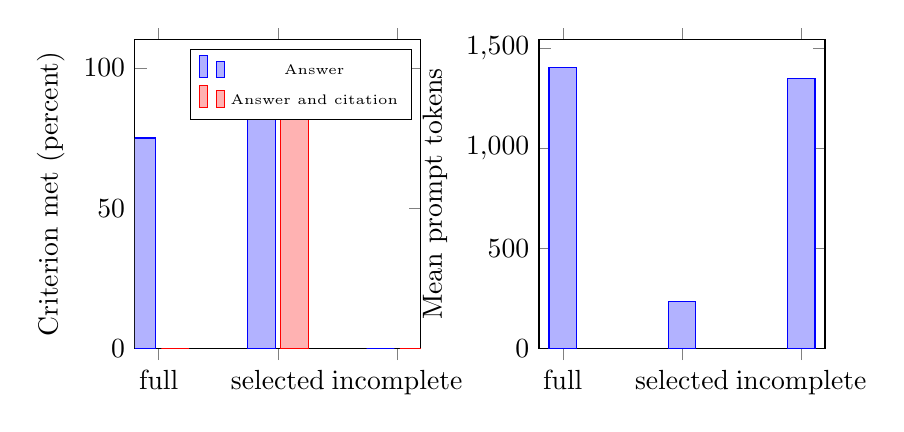
\begin{tikzpicture}

\begin{groupplot}[group style={group size=2 by 1,horizontal sep=1.5cm},width=.43\linewidth,height=5.5cm,legend style={font=\tiny}]

\nextgroupplot[ybar,ylabel={Criterion met (percent)},symbolic x coords={full,selected,incomplete},xtick=data,ymin=0,ymax=110,legend pos=north east]

\addplot coordinates {(full,75.0) (selected,100.0) (incomplete,0.0)};

\addlegendentry{Answer}

\addplot coordinates {(full,0.0) (selected,87.5) (incomplete,0.0)};

\addlegendentry{Answer and citation}

\nextgroupplot[ybar,ylabel={Mean prompt tokens},symbolic x coords={full,selected,incomplete},xtick=data,ymin=0]

\addplot coordinates {(full,1403) (selected,233) (incomplete,1351)};

\end{groupplot}\end{tikzpicture}

\par\small\textit{Figure 2. Context sensitivity and complete prompt length in the local small-model pilot. The selected package is supplied by an oracle. Both harnesses return identical paired outputs; the incomplete condition evaluates abstention.}\end{center}

\section{Results: Reliability and Scripted Applications}

The model battery creates 48 Shepherd sessions, of which 43 finish and five fail because the adapter rejects a capped completion. Every terminal session repeats without a new transport call and preserves the same terminal result. Closing and reopening preserves all 48 results; importing the archive preserves all 48 again. Original and imported stores report no integrity issues across 145 records, 144 append intents, and 48 owners. No blobs or cuts are present in this battery. These checks demonstrate terminal evidence retention for this workload, not an estimate of failure probability under an operational workload.


The terminal-reuse check intentionally includes failed invocations, so a failed model request is retained rather than silently treated as a successful answer. However, the experiment compares terminal result values and counters, not the complete canonical failure object, and null equality is weak for failed results. Full failure-record comparison and process-kill recovery during an actual local-model request are not part of this pilot. The independent whole-store integrity check provides additional structural evidence, not a semantic proof of all failure behavior.


Four offline application fixtures complete after correcting a study-runner argument error. Table 7 reports compared-side calls and retained steps. Counterfactual optimization uses 34 versus 48 scripted provider steps while retaining 48 steps on both sides; trajectory compression retains two versus four steps with one versus four live-in-session scripted provider steps. The report's application-side comparison excludes some whole-run work, such as compressor and verifier children; its full manifest costs are retained separately. Tree-RL compares roots plus branches against its own roots, so the generation budgets are unequal. No training or live proposer result is inferred.


The first study collection attempt passed an extra artifacts field to runApplicationEvaluation and was refused before execution. The runner was corrected to pass only bind and definition; the fresh report is saved separately from the original journal entry. This was a study-harness error, not a measured runtime failure. Initial module-import and sandbox connectivity setup errors likewise are excluded from the task battery; the completed marker fixes the 96-call denominator. The six-call smoke battery remains available to audit setup and cache warming.


Focused benchmark, application, provider-conversation, and compression-crash checks pass 35 tests with no skips. A complete sandboxed verification run reports 1,340 tests, 1,331 passes, two failures, and seven skips, and misses the 100\% coverage gate. With host access, the same repository suite reports 1,338 passes, no failed tests, and two skips, with 100\% line, branch, and function coverage. The skips are an absent telemetry decoder and the optional commercial-provider cache-after-rewind test. The host verification command initially stops at its final packaged-README link check because this study's guide was not yet present. After creating that guide, the packaged CLI gate passes, including a fresh installed runtime and quickstart. The full command's initial nonzero status is retained; all constituent gates have successful evidence across that run and the targeted packaging rerun.


\begin{center}\small

\textit{Table 7. Scripted application fixtures: compared-side provider calls and retained steps. Counts do not include every whole-run activity; Tree-RL budgets are unequal.}\[6pt]

\begin{tabularx}{\linewidth}{XXXXXX}

\toprule

\textbf{Application} & \textbf{Baseline} & \textbf{App calls} & \textbf{Base calls} & \textbf{App steps} & \textbf{Base steps} \\

\midrule

coding-supervisor & no\_supervision & 2 & 1 & 2 & 1 \\

counterfactual-optimization & full\_replay & 34 & 48 & 48 & 48 \\

trajectory-compression & no\_compression & 1 & 4 & 2 & 4 \\

tree-rl & flat\_grpo & 26 & 10 & 30 & 10 \\

\bottomrule\end{tabularx}\end{center}

\section{Discussion}

The local kernel's sub-millisecond append and millisecond-level prefix and subscription work support the feasibility of retaining fine-grained execution evidence under this fixed load. Archive operations and whole-store verification have substantially larger costs. This separation is useful for operational design: frequent trace events and occasional archival workflows impose different latency expectations. The present data do not establish a scaling law for larger stores, concurrent writers, network storage, or a different synchronization mode.


The scope results show why physical substrate claims must be separated from public runtime semantics. A cheap copy-on-write primitive can coexist with an expensive integrity-verified API. Both measured backends have world-dependent public latency, and clone is slower in the fork cells. Storage efficiency remains unresolved because the volume-delta measure produced implausible zeros and coarse changes. The study therefore supports a latency observation while declining a precision storage claim from the same run.


Durable traces provide inspectability and retained outcomes; they do not improve a model's evidence selection when the supplied request is held fixed. The matched harness comparison makes this distinction observable. Context selection is the intervention that changes quality in the pilot, while Shepherd provides an execution record for investigating the result. The full-context answer/citation discrepancy shows why provenance-sensitive task evaluation should not stop at answer strings.


The selected treatment is an oracle upper-bound construction for this battery. A deployed context-engineering system must discover relevant evidence, preserve conflicting versions and constraints, handle later tool outputs, and account for retrieval or summarization costs. Omitting evidence can reduce prompt size while destroying answerability, as the incomplete condition illustrates. A reliable runtime can faithfully retain an incorrect output; independent task verification and runtime integrity answer different questions.


\section{Threats to Validity}

Internal validity: the host is busy and uncontrolled; kernel repetitions share one process; suite and task order are fixed except for pair alternation; cache state is not reset; the smoke experiment can warm caches; and the active model context window is not pinned. Harness pair requests and outputs match exactly, but end-to-end latency differences remain vulnerable to cache and order. Store creation, oracle context preparation, and post-run reliability checks are outside the timing boundary.


Construct validity: terminal completion, exact answer accuracy, cited-evidence correctness, and byte-level restoration are distinct constructs. The single-call task battery is not an autonomous coding benchmark. The citation criterion is strict and intentionally penalizes distractor or obsolete evidence. Oracle selection confounds smaller size with better relevance. The digest checks cover files and names, not every metadata attribute or future process observation. Terminal-result equality after failure does not fully compare failure metadata.


Measurement validity: free-space deltas fail plausibility checks and cannot support precise storage savings. Device-layer scripts retain summaries rather than all samples. Prompt bytes differ from tokens; uncached input differs from total prompt length. Empirical p95 from ten or twelve samples is the maximum and has weak tail-estimation meaning. Normalized usage is absent on some rejected completions, so token accounting uses retained raw server usage to include failures. API cost remains unknown.


External validity: one Apple Silicon/APFS host, one 0.5B quantized model, eight simple synthetic tasks, two seeds, no multi-turn tool policy, and no independently implemented framework comparator constrain generality. No Windows, bare-metal Linux, x86-64, cloud sandbox, paid provider, coding-agent leaderboard, learning gain, security proof, or external review is established. Current source behavior and historical audit findings are not merged into a single unsupported coverage percentage.


Statistical conclusion validity: within-session dispatch events and task-seed repeats are clustered. A conditional bootstrap over eight hand-designed tasks indicates sensitivity within this battery, not random sampling from a task population. Zero observed restoration failures does not justify a production reliability guarantee. One SLO miss does not locate a root cause; passing other budgets does not establish optimality.


\section{Follow-up Experimental Protocol}

A confirmatory systems experiment should repeat complete scope trials in separate processes on an isolated host, include independently measured load and cache state, and randomize or counterbalance backend order. Storage measurements should use an isolated volume or verified extent accounting with explicit clone-sharing semantics. The copy-branch assertion must be diagnostically resolved before reporting storage ratios. Platform-specific overlay and container measurements require their actual execution environments and must retain successful probes and constituent-specific recovery evidence.


An independent-framework study should pin an upstream Python Shepherd or another harness version, define a common executable task adapter, and hold model, evidence policy, tools, timeout, retry budget, and judge fixed. Comparisons must either match durability and restoration guarantees or disclose which extra work is being purchased. Both application-level end-to-end latency and runtime-only overhead should be measured. External framework installation and execution remain unperformed prerequisites, not implicit results of the present direct-harness control.


A model-quality study should add multiple models, randomized evidence placement, multiple task families, longer tool-use trajectories, and independent executable outcome checks. A production context experiment should measure retrieval recall and precision, conflicting-version retention, summary faithfulness, and the full cost of preparing context. Failure injections should exercise malformed tool calls, output limits, cancellation, transport loss, store reopen during an unfinished session, and stale leases without weakening assertions. Local terminal retention should then be supplemented with in-flight recovery and side-effect evidence at the appropriate production seams.


\section{Conclusion}

This single-host study finds efficient durable kernel operations under the configured synthetic load and exact retained-result reuse in a small live local-model battery. It also records a real scope latency-budget miss and a failed storage-measurement assertion. Those negative findings limit the claims rather than disappear from the report. The matched direct and Shepherd harnesses have identical task outputs; relevant-evidence selection, not tracing alone, changes the quality result. The appropriate conclusion is bounded evidence for durable execution, diagnosable model behavior, and context sensitivity, with independent-framework comparison and broader agent-quality evaluation still requiring harmonized experiments.


\section{Reproducibility and Artifact Availability}

The artifact directory is .plan/benchmarks/2026-10-05. run-study.mjs invokes existing system benchmark APIs and scripts; run-agent-study.mjs performs the matched model pilot. study.config.json and agent-study.config.json specify procedures and tasks. raw/provenance.json records the initial source revision, working-tree status, runtime diff, and SHA-256 hashes of exact configuration snapshots. Kernel and scope artifacts carry their own canonical configuration digests. Different hash procedures are labeled rather than compared as if interchangeable.


analysis.py independently validates configuration snapshot hashes, recomputes summaries and task grades, checks paired requests and outcomes, exports CSV tables, and produces the two scientific figures. The native SQLite store and its portable JSON archive retain the model experiment. Smoke observations have a separate directory. Raw measurements are excluded only from automatic formatting to preserve captured bytes; research scripts and authored configuration remain linted. README.md gives exact commands and advises using fresh output directories.


All measurements and failure evidence are local artifacts. No upstream benchmark number is inserted into a result table. Related-work notes provide primary-source links and comparison-feasibility details. The report is an internally generated technical study, not a peer-reviewed publication or external audit. No runtime change is made to turn an observed failure into a pass.


\begin{thebibliography}{99}

\bibitem{ref1} Simon Yu et al. (2026). Shepherd: Enabling Programmable Meta-Agents via Reversible Agentic Execution Traces. arXiv:2605.10913v3, 24 June 2026. \href{https://arxiv.org/html/2605.10913v3}{Primary source}.

\bibitem{ref2} Shepherd TypeScript repository. Source revision d7f957caacd1e57e40417d42587618f702b5e8ca; normative performance, replay, provider, checkpoint, and evaluation documents. \href{https://github.com/avnionur/shepherd-typescript/tree/d7f957caacd1e57e40417d42587618f702b5e8ca}{Primary source}.

\bibitem{ref3} Shepherd experiments repository. Inspected revision c12ebd1b774cf12f70ef2b4486e61e7052f3e3ab; framework-performance procedures and dependencies. \href{https://github.com/shepherd-agents/shepherd-experiments/tree/c12ebd1b774cf12f70ef2b4486e61e7052f3e3ab/exp/framework-perf}{Primary source}.

\bibitem{ref4} Yang Li et al. (2025). AgentGit: A Version Control Framework for Reliable and Scalable LLM-Powered Multi-Agent Systems. arXiv:2511.00628v1, 1 November 2025. \href{https://arxiv.org/abs/2511.00628v1}{Primary source}.

\bibitem{ref5} Xingyao Wang et al. (2026). The OpenHands Software Agent SDK: A Composable and Extensible Foundation for Production Agents. arXiv:2511.03690v2, 22 April 2026. \href{https://arxiv.org/abs/2511.03690v2}{Primary source}.

\bibitem{ref6} Cong Wang and Yusheng Zheng (2026). Fork, Explore, Commit: OS Primitives for Agentic Exploration. arXiv:2602.08199v2, 19 March 2026. \href{https://arxiv.org/abs/2602.08199v2}{Primary source}.

\bibitem{ref7} Jiakai Xu et al. (2026). StateFork: Branchable Infrastructure for Agent Exploration. arXiv:2609.38648v1, 29 September 2026. \href{https://arxiv.org/abs/2609.38648v1}{Primary source}.

\bibitem{ref8} SQLite documentation. Write-Ahead Logging and PRAGMA synchronous. Official durability semantics. \href{https://sqlite.org/pragma.html#pragma_synchronous}{Primary source}.

\bibitem{ref9} Ollama documentation. OpenAI API compatibility, response format, seed, and sampling controls. Consulted 5 October 2026; measured server version 0.35.1. \href{https://github.com/ollama/ollama/blob/main/docs/api/openai-compatibility.mdx}{Primary source}.

\end{thebibliography}\end{document}
